\documentclass[nofootinbib,aps,pre,twocolumn,superscriptaddress,showkeys,showpacs]{revtex4-1}
\usepackage[capitalize]{cleveref}
\usepackage{amsmath, amsthm, amssymb}
\usepackage[toc,page]{appendix} 
\usepackage{graphicx}
\usepackage{subfigure}
\usepackage{wrapfig}
\usepackage{color}
\usepackage{lipsum}% http://ctan.org/pkg/lipsum
\usepackage{graphicx}% http://ctan.org/pkg/graphicx
\begin{document}

\title{Catchy Title Goes Here}
\author{Laura Sampson}
\affiliation{Center for Infectious Disease Dynamics, Pennsylvania State University, State College, PA, 16801}
\author{Matthew Ferrari}
\affiliation{Center for Infectious Disease Dynamics, Pennsylvania State University, State College, PA, 16801}

\begin{abstract}


\end{abstract}
\maketitle

\section{Introduction \label{sec:Intro}}
Dramatic improvements in the coverage of vaccination with measles-containing vaccines have lead to significant reductions in the incidence of measles disease and the associated childhood mortality ~\cite{perry_global_2014}. Despite these improvements at the national scale, however, significant heterogeneity in both vaccination coverage and disease incidence remains at the sub-national level~\cite{prada_demographics_2017,takahashi_geography_2017,metcalf_transport_2015}.
Given the high transmission rate of measles, the proportion of the population that must be immunized to achieve and maintain elimination of measles is likely to be greater than 90\% in most populations [REF - Goodson?] (the exact level will be modulated by locally specific conditions such as population density and contact rates).
%"The WHO recommends that programs use good quality data to monitor population immunity by identifying and responding to large numbers of susceptibles" from Winter et al reference to WHO Measles vaccines: WHO position paper Wkly Epidemiol Rec 2017;92:205-28
%"Because the risk of measles outbreaks is determined by the rate of accumulation of susceptible people in the population, programmes should use available good quality data on population immunity (i.e. vacci- nation coverage, surveillance, serological studies) to monitor the accumulation of susceptible people and conduct follow-up campaigns before the number of pre-school children susceptible to measles approaches the equivalent of one birth cohort, in order to prevent an outbreak of measles. This approach has been found to be programmatically useful in preventing large outbreaks. However, for large countries and countries which are close to measles elimination, a more exten- sive assessment of the accumulation of susceptible persons should be carried out at the subnational level." WHO Measles vaccines: WHO position paper Wkly Epidemiol Rec 2017;92:205-28 -- http://apps.who.int/iris/bitstream/handle/10665/255149/WER9217.pdf?sequence=1

The size and age-distribution of the population susceptible to measles (hereafter we refer to this as the "susceptible persons") depends on the competing processes of susceptible recruitment through birth and susceptible loss through either natural infection or vaccination. 
Quantifying the size and age distribution of susceptible persons to measles is a critical tool in evaluating outbreak risk, the performance of vaccination programs, and developing vaccine-based interventions. The WHO recommends that programs monitor the accumulation of susceptible persons using "good quality data" for all countries, and that these should be made at the sub-national level for large countries and those close to measles elimination [REF -- Wkly Epid Rec].

Direct observation of the distribution of susceptible persons is challenging as it requires a sero-survey which can be cost-prohibitive. 
Moreover, while a sero-survey can provide a well resolved cross-sectional estimate of the distribution of susceptible persons, it cannot, by itself, quantify the relative contribution of natural and vaccine-derived immunity as current serological diagnostics cannot distinguish between these two sources~\ref{Winter2018Sero}. Fortunately, the relative contribution of these sources can be estimated through modeling. 

In the absence of a sero-survey, the number and age-distribution of susceptible persons can be estimated though demographic models that account for inputs through births and immunization via both vaccination and natural infection~\cite{METCALF2017S14,TRENTINI20171089,Winter2018Sero}. In this approach, the contribution of natural immunity is modeled as the result of a dynamic transmission model [REF] which requires explicit assumptions about the age-specific force of infection via a Who Acquires Infection From Whom (WAIFW) matrix that describes the age-specific rate of infectious contacts from each age class to each of the others.  Direct estimation of this WAIFW matrix is challenging from disease incidence or seroprevalence data (though see Whittaker and Farrington etc.), and thus it is common to make simplifying assumptions that either the WAIFW matrix is constant for all ages (i.e. a uniformly well-mixed system) ,or that the WAIFW matrix is a scalar function of some other measurable interaction process, such as contacts measured via diary studies~\ref{Polymod}.

The catalytic model is another approach that was initially proposed as a method for estimating the age-specific force of infection from cross-sectional, age-specific sero-prevalence data~\cite{griffiths_catalytic_1974}. 
This model, which represents the probability of immunization via natural infection at a specific age, $a$, as the cumulative sum of age-specific force of infection prior to this age, was then adapted by Grenfell and Anderson~\cite{Grenfell1985} for use with cross-sectional, age-specific case observations.  
The resulting fitted model can then be used to estimate the age-specific distribution of susceptible persons.
Thus, in the absence of a sero-survey it is possible to estimate seroprevalence from routinely collected age-specific case reporting.

Original applications of the catalytic model assumed that natural infection was the only source of immunity~\cite{griffiths_catalytic_1974}.  
In the vaccine era, however, the age distribution of susceptibility is generated by the sum of the rates of vaccination and natural infection. 
Though measles vaccination is recommended to follow a specific schedule, with children receiving two doses at prescribed ages, in practice, the ages at which children receive an immunizing dose of measles containing vaccine (MCV) may be highly variable because of variation in access to vaccination services~\cite{METCALF2017S14,TRENTINI20171089,Winter2018Sero} and the multiple vaccination initiatives that are employed: e.g. routine vaccination, supplementary immunization activities, child and maternal health days, school-based immunization drives, etc.
Recent work has highlighted significant variability both in the maximum vaccination coverage achieved and the timeliness of vaccination - that is, the proportion of children receiving vaccination at any given age. Thus, vaccination can itself be modeled as an age-specific hazard rate that accounts for the sum of multiple forces.
Failing to account for the age-specific pattern of vaccination may lead to a biased interpretation of case-data, as children who might be vaccinated later than the recommended age remain susceptible and may contribute to incident cases. 

An additional complication is that vaccination does not necessarily imply immunization.  
In developing-world settings, the efficacy of measles vaccine is often assumed to be $\sim 85 \%$ , though it is known to improve with age as older children are more likely to have lost maternally transferred antibodies~\cite{Uzicanin2011}. The effectiveness of vaccine delivered in field settings may also vary dramatically due to stability and effectiveness of the vaccine cold chain~\cite{Doshi2017}.  
A comparison of the age-distribution of vaccination and sero-prevalence may highlight areas with low effectiveness, and absent a sero-survey this assessment could be made using age-specific case records.

Here we present an extension of the catalytic model that represents the age-specific proportion immune as the cumulative sum of the hazards of both natural infection (force of infection) and effective immunization via vaccination.
We illustrate how this model can be used to estimate the age-specific sero-prevalence,  the age-specific rates of vaccination and force of infection, and vaccine effectiveness using age-specific vaccine coverage data and case-records. 
We illustrate performance of this model using both simulated data and measles case surveillance data from DRC combined with vaccination coverage surveys conducted as part of the 2013-14 DHS.  
A contemporary measles sero-survey conducted during the 2013-14 DHS allows us to validate the performance of our estimates of sero-prevelence against direct measurements. 
We finally present a fit of the model to the surveillance data, vaccine coverage data, and sero-survey and discuss opportunities for combining data sources.


\section{Methods \label{sec:Methods}}
\subsection{Competing Rates Model \label{subsec:CompetingRates}}
The classic catalytic model for disease infection, developed in the late 1950's, gives the probability of immunity at age $a$ as
\begin{equation}
p(\mathrm{immune}|a) = 1 - \exp\left(-\int_0^a f(a') da'\right),
\label{eq:CatMod}
\end{equation}
where $f(a)$ is the \emph{force of infection} at age $a$, which can be thought of as the rate of infection at a particular age. This expression is valid in the absence of vaccination, as in this case infection is the only source of immunity. In the case of measles, this expression gives the probability of an individual at age $a$ being seropositive for measles.

In situations in which vaccination is present, vaccination provides a second means of acquiring immunity - the `force of vaccination,' or `vaccination hazard' (vh). If we represent this as $v(a)$, then we can extend Eq.~\ref{eq:CatMod} to give the probability of an individual testing seropositive at age $a$ as
\begin{align}
p(\mathrm{immune}|a)  &= 1 - \exp\left( - \int_0^a f(a') + v(a') da'\right) \nonumber \\ 
&=1 - \exp\left(-\int_0^a f(a') - \int_0^a v(a') da'\right).
\label{eq:CatModSum}
\end{align}

The functional forms of $f(a)$ and $v(a)$ are free to be specified. In this study, we choose to use un-normalized Weibull distributions to parameterize both of these functions, as they have been shown to be sufficiently flexible to match a range of possible forces of infection and vaccination hazards~\cite{ferrari_episodic_2010}. Thus $f(a) \rightarrow f(a|\mathbb{\psi})$ and $v(a) \rightarrow v(a|\mathbb{\theta})$, where $\mathbb{\psi}$ and $\mathbb{\theta}$ are vectors of the parameters we use for the Weibull distribution - height ($\eta$), scale ($\alpha$), and shape ($\beta$). This gives six parameters that fully specify the forms of $f(a)$ and $v(a)$ from Eq.~\ref{eq:CatModSum} - $\alpha$, $\beta$, and $\eta$ for two independent Weibull distributions. To allow for the fact that not all vaccinations produce immunity, we introduce a seventh parameter - the vaccine effectiveness ($\gamma$). This enters the equation as a multiplier on $v(a)$ that ranges between $0.0$ and $1.0$.

Besides the flexibility of the distribution, another appealing aspect of the Weibull as our choice of parameterization is that it can be integrated analytically, as
\begin{equation}
\int_0^a g(a';\eta,\alpha,\beta) = \frac{\beta}{\alpha} \eta \left( 1 - \exp(-(x/\alpha)^\beta) \right).
\end{equation}
We re-absorb the factor of $\beta/\alpha$ on the r.h.s. of this equation into the parameter $\eta$, and have a final expression for the probability of immunity at a particular age
\begin{align}
\label{eq:seroprob}
p(\mathrm{immune}|a) = 1 - \exp\big\{&-\eta_f\left(1-\exp(-(a/\alpha_f)^{\beta_f})\right)  \nonumber \\ 
&-\eta_v \gamma \left(1-\exp(-(a/\alpha_v)^{\beta_v}) \right)  \big\},
\end{align}
which is parameterized by seven total parameters - $\{\eta_f, \alpha_f, \beta_f, \gamma, \eta_v, \alpha_v, \beta_v\}$.

This is the model that we use to analyze simulated data (see Sec.~\ref{subsec:simdata}), but we found after initial exploration using the data from the Democratic Republic of Congo that the resulting foi was qualitatively quite flat, and so we decided to extend this model by adding a constant to the force of infection as
\begin{equation}
\rm{foi}(a) = \omega * \rm{Weibull} + (1 - \omega)*\kappa,
\end{equation}
where $\omega$ ranges between $0$ and $1$, and determines the relative weighting of the Weibull and constant terms, and $\kappa$ is a constant that is allowed to range between $10^{-4}$ and $10^2$. The expression in Eq.~\ref{eq:seroprob} is then trivially updated to reflect the integral of this more complicated force of infection function. We use Bayesian model selection, discussed in Sec.~\ref{subsec:BF}, to determine for which provinces this more complicated model is appropriate.

Eq.~\ref{eq:seroprob} gives the probability of observing a seropositive individual at age $a$, which accounts for one of our three datasets. The other two are vaccination data and case data. Using the function described above for vaccination hazard, the probability of an individual having been vaccinated by age $a$ is given by
\begin{equation}
p(\mathrm{vaccinated}|a) = 1 - \exp \left\{ - \eta_v (1-\exp\left(-(a/\alpha_v)^{\beta_v}\right) \right\}.
\end{equation}
Finally, the probability of an individual being recorded as a case at age $a$ is the force of infection at that age multiplied by the probability that an individual is susceptible at that age. The probability of susceptibility is of course $1 - p(\mathrm{immune}|a)$, and so the probability of observing a case at age $a$ is
\begin{widetext}
\begin{equation}
p(\mathrm{case}|a) = \left\{ 1 - \exp\left[ -\eta_f \left( \frac{\beta_f}{\alpha_f}\right)\left(\frac{a}{\alpha_f}\right)^{\beta_f - 1}\right] \exp\left[ (a/\alpha_f)^{\beta_f}\right] \right\}
\times \left\{ 1-p(\mathrm{immune}|a)\right\}.
\end{equation}
\end{widetext}

The data we work with (described in detail in Sec.~\ref{subsec:Data}) consists of the number cases as a function of age (in years), serology tests and results as a function of age, and vaccination status as a function of age for a sample of individuals within a particular province. The likelihood for observing this dataset given values for the model parameters as
\begin{align}
\log \mathcal{L} (\mathbf{c}, \mathbf{v_t}, \mathbf{v_o}, \mathbf{s_t},&\mathbf{s_o}|\eta_f, \alpha_f, \beta_f, \gamma, \eta_v, \alpha_v, \beta_v)\nonumber \\ 
& = \sum_aB\left(v_o(a), v_t(a); p(\mathrm{vaccinated}|a)\right) \nonumber \\
&+ \sum_a B\left(s_o(a),s_t(a);p(\mathrm{immune}|a)\right) \nonumber \\
&+ M\left(\mathbf{c};p(\mathrm{case}|a)\right),
\label{eq:loglike}
\end{align}
where $s_t$ is the total number of individuals tested for IgM seropositivity, and $s_o$ is the number of positive tests; and $v_t$ is the number of individuals surveyed about vaccination status, while $v_o$ gives the number who have been vaccinated. $B$ represents a binomial probability, and $M$ represents a multinomial distribution, and the sums are over age classes. As noted, each data point includes the age of the individual in question.

\subsection{Model Comparison\label{subsec:BF}}
For the real data from the DRC, we wish to determine which provinces warrant the more complicated seroprevalence model from Sec.~\ref{subsec:CompetingRates} that includes a constant in addition to the Weibull function, and which are described sufficiently by a constant force of infection alone. To do this, we calculate the Bayes factor (essentially the betting odds) between the two models, which, given that our prior belief in the two models is equal, is simply the ratio of the evidence for each of the models~\cite{TheRev}. The evidence is the fully marginalized likelihood (FML), and can often be quite difficult to calculate accurately. Luckily for us, the two models in question are nested - we recover the constant-only model when $\alpha = 1.0$ -  and so we can use a technique called the Savage-Dickey density ratio.

Two models, $\mathcal{M}_0$ and $\mathcal{M}_1$, where $\mathcal{M}_0$ is the simpler model, are nested when there exists a parameter $\omega$ for which $\mathcal{M}_0 = \mathcal{M}_1$ when $\omega = \omega_0$. (For us, constant is the same as Weibull plus constant when the parameter $\alpha$ is equal to 1.0). In this case, the Bayes factor between $\mathcal{M}_0$ and $\mathcal{M}_1$ is simply
\begin{equation}
BF_{01} = \frac{\rm{posterior}(\omega =\omega_0)}{\rm{prior}(\omega=\omega_0)},
\end{equation}
where posterior() and prior() refer to the posterior and prior densities at $\omega = \omega_0$. To evaluate this quantity, it is only necessary to generate the posterior distribution of $\omega$, and then compare the posterior and prior densities.

We generate these distributions for each province independently using Markov chain Monte Carlo techniques, described in the next section, and find that only three provinces are adequately described by the constant force of infection model:  Bas Congo, Kasai Occidental, Kasai Orientale, and Maniema. The rest of the provinces require the more complicated Weibull plus constant model. For all of the results presented in Sec.~\ref{sec:Results}, we use these models as noted here for each of the provinces, except for Equateur. In Equateur, the more complicated model was preferred when fitting all three datasets, but the constant only model was preferred when fitting only case and vaccination data, and so these models were used accordingly.

\subsection{MCMC Sampler \label{subsec:MCMC}}
Given our set of model parameters and the definition of the likelihood in Eq.~\ref{eq:loglike}, we can generate samples of the posterior distributions of the model parameters using Markov chain Monte Carlo (MCMC) techniques. We use the \texttt{PTMCMC} sampler package in Python~\cite{PTMCMC}, which incorporates parallel tempering, differential evolution, and proposals along the eigenvectors of the covariance matrix. This sampler is described in detail in ~\cite{Arzoumanian2014}.

We must specify prior distributions on each of our model parameters before running. These are listed in Table~\ref{table:priors}. 
\begin{table}
\begin{center}
\begin{tabular}{ c|c }  
Parameter & Prior \\
 \hline
 $\alpha_v$, $\alpha_f$ & $\Gamma(2,500)$ \\ 
 $\beta_v$, $\beta_f$ &$ \Gamma(2,5)$ \\ 
 $\eta_v$, $\eta_f$&$ \Gamma(2,15)$ \\ 
 $\gamma$ & $\beta(16,5)$ \\
 \hline
\end{tabular}
\caption{Prior distributions for the seven model parameters. $\Gamma(a,b)$ is the gamma distribution with shape $a$ and scale $b$, and $\beta(c,d)$ is the $\beta$ distribution with shape parameters $c$ and $d$. \label{table:priors}}
\end{center}
\end{table}

We run for $150000$ iterations, keeping every $100$th point after a burnin period of $5000$ steps in order to decrease autocorrelation. The two-dimensional posterior distributions for the parameter pairs are shown in Appendix~\ref{app1}.

\subsection{Simulated Data\label{subsec:SimData}}
To confirm that we can accurately recover the force of infection and vaccination hazard using the model we have chosen, we generate simulated datasets consisting of age-specified measles case, vaccination, and serology data using a previously developed, age-structured MSIRV (Maternally immune, Susceptible, Infected, Recovered, Vaccinated) model~\cite{Metcalf2012}. We used demographic parameters from UN estimates for the DRC and increased vaccination linearly from 0 to 50\% over the first 30 years of a 50 year simulation. $R_{0}$ (the number of secondary cases resulting from the introduction of a single infected individual) was assumed to be constant at 15 over the entirety of the simulation. The force of infection (foi) was not directly chosen to be a Wiebull function, but is generated using the specified $R_0$ and WAIFW (Who Acquires Infection from Whom) matrix that describes social interactions as estimated via the POLYMOD study~\cite{Polymod}. This means that we cannot directly compare the recovered Weibull parameters to injected parameters, but we \emph{can} compare the recovered foi curve to the true values, as well as the recovered vaccination efficacy ($\gamma$) to the true value. 

While the raw MSIRV model output always entails a value for $\gamma$ of 1, we can simulate scenarios in which $\gamma$ is lower by drawing false positive vaccination responses from a binomial distribution with the corresponding probability, and adding these to the vaccination data generated from our simulation. For example, given that our simulation has a maximum vaccination rate of 50\%, we can simulate a $\gamma$ of 0.75 by assuming that, on average, 67\% of individuals in a given age class will report that they have been vaccinated.

After we generated a full time-series of case, vaccination, and serology data, we then downsampled the simulation results by randomly drawing the same number of observations as are present in the empirical data from the DRC.

\subsection{Data \label{subsec:Data}}
The real-world data that we apply our model to is from the Democratic Republic of the Congo (DRC), aggregated by province. We note that DRC changed from an 11 province system to a 26 province system in 2015; here we use the 11 province designations. For each province, we have three data sets: vaccination coverage, seroprevalence, and case data, all broken down by age. 

The vaccination coverage data is from age-specific survey responses from the 2013-2014 Demographic and Health Survey (DHS) made publicly available by ICF International (The DHS Program - Data Available at http://dhsprogram.com/Data/). The survey contains one record for each interviewed woman's child below 5 years of age at the time of the survey.   For each child we extracted the age, in months, at the time of the survey and whether or not the child had ever been vaccinated for measles, based on either the record on a vaccination card or parent/guardian recall. We note that parental recall of vaccination may suffer from biases, particularly for older children. Further, the DHS survey question did not distinguish between different sources of measles vaccination (e.g. through routine program, supplemental vaccination campaigns, or outbreak response vaccination campaigns).  However, as vaccination cards were rarely available in this survey, parental recall allows the inclusion of many more survey responses; in the 2013-14 DHS in DRC only 1436 respondents had a clearly marked vaccination card, out of 10366 children. Parental recall has previously been show to provide a relatively robust indicator of vaccination status\cite{ndirangu_validating_2011}. Administered measles vaccines have shown to be highly effective in generating protective immunity\cite{guris_measles_1996,king_clinical_1991}, and we characterize our vaccine effectiveness parameter $\gamma$ as the probability that a child reported as vaccinated based on either a written record or parental recall was in fact vaccinated and developed protective immunity as a result. Vaccination bias may be lower than one due to recall bias in parental reporting of children's vaccination status, failure of measles vaccination in generating protective immunity, or immunity due to natural infection having already been attained prior to infection.

The seroprevalence data is from dried blood spot samples that were taken from children in a subset of households during the 2013-14 DHS survey and tested for the presence of measles IgG antibodies.  Samples were collected from 8267 children between the ages of 0 and 59 months of age. Due to inconclusive results or errors in testing 307 samples were discarded, leaving 7960 samples classified as measles IgG positive or negative. As with the vaccination responses, each sample was geolocated to the cluster-level and we aggregated all samples within each of the 11 provinces.

The age distribution of measles cases was taken from individual case-reporting for DRC reported to the World Health Organization (WHO) between 2011-2017. During this time period, 33098 suspected measles cases were reported, of which 5495 were classified as lab-confirmed by the presence of IgM measles antibodies and 13858 were classified  as epidemiologically linked because they occurred close in time and space to a lab confirmed case.  For each suspected case we extracted the age, in months, and the province in which the case was recorded. Because the age of many cases was binned to the year (e.g. recorded as 24 or 36 months) we rounded all cases up to the nearest year; thus cases were binned into 1 year age classes following the convention (0,1],(1,2], etc. 

\subsection{Comparing Data and Inference \label{subsec:Comp}}
A standard approach for interpreting the results of Bayesian inference would be inspecting the posterior distributions for the model parameters. But the parameters of our model are not, in themselves, particularly interesting - it is the inferred seroprevalence, case distribution, and vaccination probability that we wish to compare with the data. To do this, we generate the posteriors on $\{\eta_f, \alpha_f, \beta_f, \gamma, \eta_v, \alpha_v, \beta_v\}$ as described, and then draw from these posteriors to generate the seroprevalence, case, and vaccination curves as laid out in Sec.~\ref{subsec:CompetingRates}. Because the vaccine efficacy, $\gamma$, is of interest on its own, we also examine the posterior distributions for this parameter in detail.

In order to assess the impact of different types of data (case, serology, and vaccination data) on our inferences, we run the MCMC package described in Sec.~\ref{subsec:MCMC} on the vaccination and case data alone, the serology and case data alone, and all three datasets together. The results of all of these analyses are discussed below.

We also assess an additional measure of the `infection risk' inferred for each province, which we define as
\begin{equation}
r = \int_0^{10} \mathrm{foi}(a) da,
\end{equation}
 or the force of infection integrated from 0 to $10$ years.  Thus, this is an aggregate measure of the total infection risk up to age 10. We calculate this infection risk using  case and vaccination data only, and all three datasets. In addition we calculate this measure using the model analyez with the serology data alone (without case or vaccination coverage data).  This latter measure reflects the estimate one would make if inference were based only on the sero-survey of children between the ages of 5-59 months.  
 
\section{Results \label{sec:Results}}
\subsection{Simulated Data \label{subsec:SimDat}}
%Although we have chosen a flexible functional form to represent the force of infection and vaccination hazards, we know that that the true functions present in nature are unlikely to be precisely matched by Weibull distributions. This will necessarily lead to some level of biases in our inferences. To understand these possible biases, we analyze simulated data with known foi, vaccination hazard, and $\gamma$ (vaccine efficacy), and examine the results.  

Using simulated age-specific case data and a simulated vaccine coverage survey, we estimated the cumulative proportion sero-positive as a function of age (Figure~\ref{fig:simplots}) under different scenarios of vaccine effectiveness (see definition in Sec.~\ref{subsecSimData}).  Using the model analyzed without using serology data, the estimated age-specific sero-prevalence was broadly consistent with the simulated sero-prevalence, though with a slight negative bias (Figure~\ref{fig:simplots} (a) - top). Similarly, the estimated cumulative probability of vaccination as a function of age was unbiased for the simulated values (Figure~\ref{fig:simplots} (a) - middle).

The Weibull distribution used to approximate the age-specific FOI is an over-simplification of the complicated age-specific mixing represented in the POLYMOD WAIFW matrix used in the MSIRV simulations; and is likely to be an over-simplification of the true, but unknown, age-specific FOI that exists in any real-world epidemiological setting.  Acknowledging that limitation, the estimated Weibull FOI broadly reflects the average age-specific FOI from the MSIRV model(Figure~\ref{fig:simplots} (b) - top) ; the latter is calculated as the product of the WAIFW matrix and the average age-specific vector of infectious cases over the full simulation.  The resulting Weibull fit, which is necessarily unimodal, tends to average over the two modes in the simulated FOI which reflect the effect of age-assortative mixing and interactions among generations (i.e. parents and children).  The estimated vaccination hazard clearly identifies the mode of age-specific vaccination and the magnitude of the vaccination hazard is positively correlated with the simulated values (Figure~\ref{fig:simplots} (b) - bottom). 

The vaccine effectiveness, $\gamma$, which measures the likelihood that a child recorded as vaccinated in a vaccine survey was immunized by vaccine, is poorly estimated using a model analyzed with only age-specific case incidence and vaccination survey data (Figure~\ref{fig:simplots} (c) - top).  The inferred values of vaccine efficacy are positively correlated with the true value used in simulation, but are biased significantly low; in simulation runs with low effectiveness, the resulting posterior estimate was low and significantly different than the prior on $\gamma$ (Figure~\ref{fig:simplots} f).  This bias is off-set by slight biases in other parameters (see Supplement), which explains why the estimated age-specific sero-prevalence only exhibited a slight negative bias. Estimated vaccine effectiveness remains biased in the corresponding model that includes seroprevalence (Eq 8); though the correlation between the posterior mean estimate and the true value used in simulation is stronger and the variance of the posterior distribution is smaller when serology data are included (Figure~\ref{fig:simplots} (c) - bottom).  Thus, while vaccine effectiveness may always be challenging to estimate, the resulting estimate from this model may serve as an indicator of vaccine effectiveness, and in particular the \emph{relative} values of vaccine effectiveness recovered for two different locations likely correctly identify the location with lower $\gamma$.  Results for the age-specific sero-prevalence, probability of vaccination, and the hazards for FOI and vaccination (e.g. corresponding to (Figure~\ref{fig:simplots}) for the model analyzed using age-specific case incidence, vaccination survey data, and seroprevalence data are presented in the Supplement.

%Figure~\ref{fig:simplots} shows the results from this analysis. In the top right panel, we show the injected (dashed lines) and recovered (solid lines) curves for the force of infection and vaccination hazard from simulated data with vaccine efficacy ranging between $\gamma = 0.9$  and $\gamma = 0.6$. The top graph in this panel shows the force of infection, and it is very clear that a Weibull distribution is not a good fit for the true force of infection, which is bimodal.  Because of this, we do not expect to be able to accurately infer the simulation parameters (i.e., $\gamma$). We examine the inferred values for this parameter in the top left panel of this same figure. 

\begin{figure*}
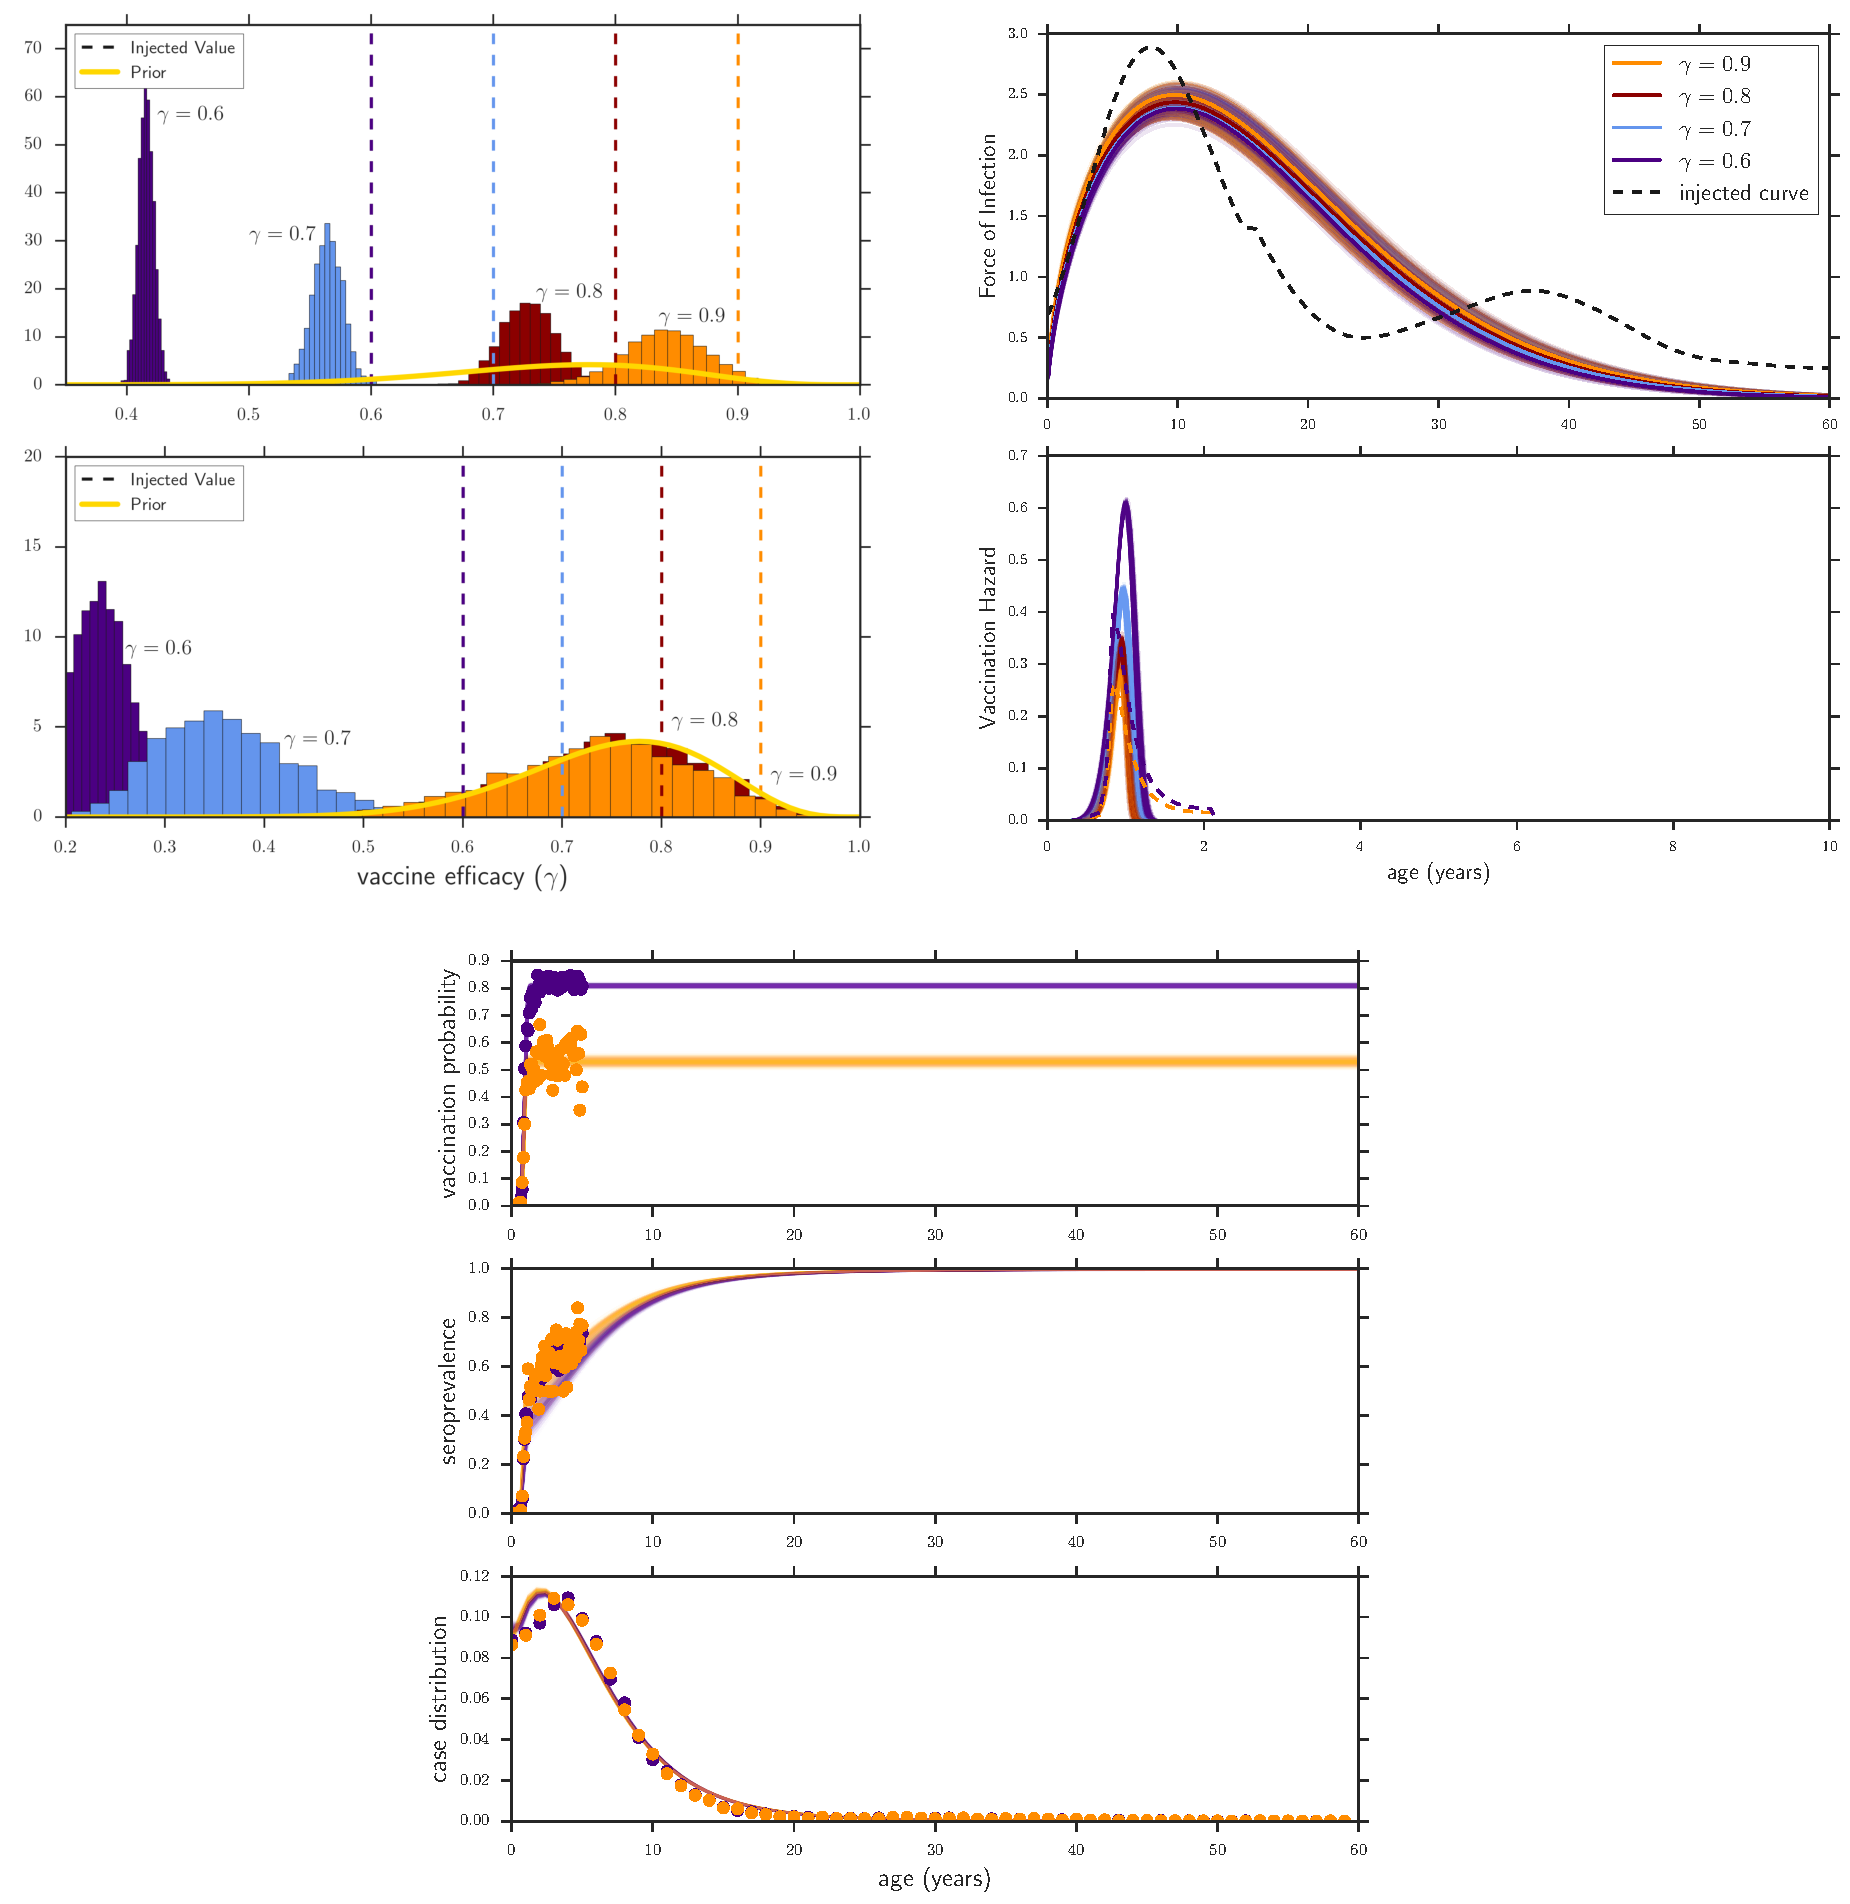
\includegraphics[width=0.9\textwidth,angle=0]{figures/SimPlots-crop.pdf}
\caption{\label{fig:simplots} Results from study using simulated data. 
The top left plot shows the posterior distributions for each of four different datasets generated with four different vaccine effectiveness ($\gamma$). The injected values are shown as dashed lines, and the recovered distributions are labelled with the associated value of $\gamma$. The prior is shown as a solid yellow line. The top panel of this plot is generated using all three datasets, and the bottom panel uses only vaccination and serology data. We find that the recovered value of $\gamma$ is typically biased low, but that the ordering of datasets by $\gamma$ is recovered correctly. In the cases of high $\gamma$ and no serology data, the recovered posteriors are dominated by the prior.
The top right plot shows the injected (dashed) and recovered (solid) force of infection (top panel) and vaccination hazard (bottom panel) for the same four datasets. The Weibull is not a good fit to the injected foi, but the resulting fits to the observable data (bottom plot) are not overly biased. The fit to the vaccination hazard is similarly not perfect, and the overly-high peaks can explain the general biasing of $\gamma$ to low values. 
The bottom plot shows the injected (points) data and recovered (lines) curves for the highest (orange) and lowest (indigo) values of $\gamma$ for seroprevalence data (top), vaccination data (middle), and case data (bottom). Solid points indicate observations between 5-59 months, the age range observed in the 2014 DHS survey, and the open points give observations greater than 59 months. }
\end{figure*}

%This panel shows the posterior distributions and assumed values for $\gamma$ from simulated datasets with four different values of $\gamma$. The top plot is generated by analyzing all three datasets, and the bottom plot using only case and vaccination data. In addition to the assumed values and the posteriors, we also show the prior on $\gamma$ as a yellow line. In the top we see, as expected, that the inferred values for $\gamma$ are systematically biased away from the injected values - they turn out to be consistently biased low in this case. Although this means that we do not necessarily infer an accurate value for vaccine efficacy with this data using this model, it is important to note that we do infer the correct \emph{ordering} for $\gamma$. That is, if these were four different locations, we would correctly identify the location with the lowest vaccine efficacy.

%The bottom plot in this same panel shows the inferred values for vaccine efficacy using only case and vaccination data - i.e. leaving out the serology data from the analysis. For the higher levels of $\gamma$, the results are dominated by the prior. For the lower values, the recovered values are again biased quite low, but also again recover the correct ranking of vaccine efficacy.

%Finally, we wish to explore the recovered fits to the true data when analyzing all of the simulated datasets. These results are shown in the bottom panel of Fig.~\ref{fig:simplots}. Here, we show the recovered (lines) seroprevalence, vaccination probability, and case distribution for simulated data with vaccine efficacy of $\gamma = 0.6$ (indigo) and $\gamma = 0.9$ (orange). The true values for each of these are shown as points. We can see that the injected data is recovered well with our model, even though the foi and vaccination hazard are not fit particularly well themselves. This is because the data are a function of the \emph{integrated} foi and vaccination hazard, which allows for some ambiguity in the details of the functions themselves. 

\subsection{Application to DRC Data \label{subsec:DRC}}
%We now turn our attention the the results of our analyses when using the real data from the DRC. As discussed in Section~\ref{subsec:BF}, we first determined which model for foi was preferred for each of the eleven provinces we used for our geographical units. We found that when all of the data was included, the only provinces that were better-described by the simple, constant-only model were Bas-Congo, Kasai Occidental, Kasai Orientale, and Maniema. When we looked at the case and vaccination data only, Equateur was also better-described by this model, and when we analyzed only the seroprevalence data, the analysis for all provinces preferred this model. 

For each of the 11 provinces in DRC, we analyzed both the constant and Weibull plus constant hazard models using age-specific case incidence and vaccination survey data, first without and then with the seroprevalence data from the 2014 DHS survey. When seroprevalence data were not included, the constant hazard model was selected as the best model (via calculation of Bayes factors) for Bas-Congo, Equateur, Kasai Occidental, Kasai Orientale, and Maniema.  When seroprevalence data were included in the model, the constant hazard model was preferred for Bas-Congo, Kasai Occidental, Kasai Orientale, and Maniema.  The age-specific seroprevalence estimated using only the case and vaccination coverage data tended to over-estimate the prevalence observed in the 2014 DHS and the estimate that resulted from the inclusion of the serology data in the model~\ref{fig:sero}.(Note that in Fig.~\ref{fig:sero} (b) and ~\ref{fig:foivaccveff} (a) and (b), provinces are split by a blank space between those for which the Weibull plus constant model was preferred, and those for which the constant-only model was better). The magnitude of this bias varied from province to province, with the largest differences observed in Bandundu, Equateur, Nord Kivu, and Sud Kivu. In each of these cases, the model using only case and vaccination survey data would have given an over-estimate of the proportion immune at each age class, and thus an under-estimate of measles outbreak risk. 

\begin{figure*}
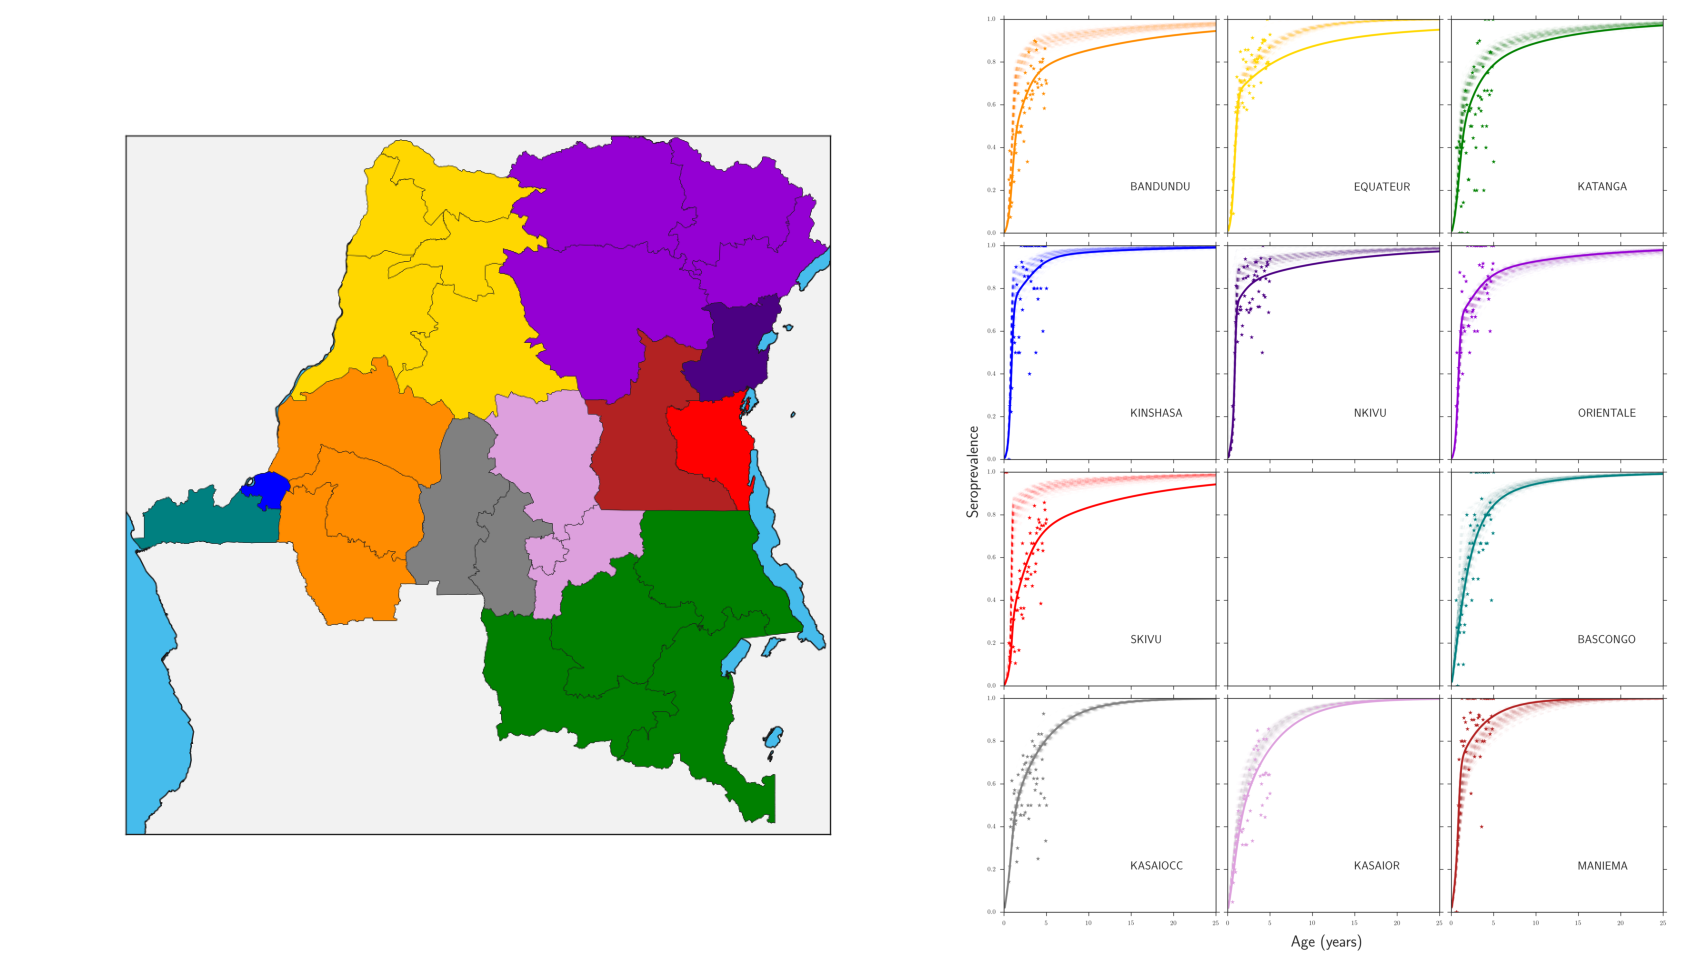
\includegraphics[width=0.85\textwidth,angle=0]{figures/SeroPlots-crop.pdf}
\caption{\label{fig:sero} Panel (a): color coding of locations used in our analysis. The data was split into the 11 provinces in existence between 1997 and 2015. The map shows these provinces in different colors, as well as the current administrative boundaries as black lines. The colors on this map correspond to the colors used for each province in all figures in this section. Panel (b): seroprevalence data (points) and inferred values up to 25 years. The solid line shows the mean of the posterior distribution for the inferred seroprevalence using all three datasets, while the dashed lines show the full range of the posterior distribution generated using only vaccination and case data. The provinces before the blank space were analyzed using the Weibull plus constant model for force of infection, while those after (starting with Bas Congo) used only a constant. For the provinces in which seroprevalence data makes a difference in the inferred values, the inferred curve is typically lower than that generated using only vaccination and case data. This is especially pronounced in Sud Kivu.}
\end{figure*}

%The left panel of Fig.~\ref{fig:sero} the color-coded provinces. We use these colors throughout this section to show the results from individual provinces. The right panel shows the recovered seroprevalence data (right panel) for all 11 provinces, using all three datasets (solid line) and the vaccination and case data only (dashed lines). The solid line is the mean of the posterior distribution generated using all three datasets, while the dashed lines show the full range of the posterior for the vaccination/case data analysis. We see that, in general, the seroprevalence data leads to a \emph{lower} estimate of seroprevalence in the population than the case and vaccination data alone. This is because the prior on vaccine effectiveness is peaked around $0.85$ - that is, when a study participant reports that they or their child is vaccinated, we give an $85\%$ probability that not only is the recollection correct, but that the vaccine produced immunity. Without seroprevalence data, there is not enough information in the datasets to pull the value for $\gamma$ away from this peak, and so we overestimate the immunity in the population. This is particularly noticeable in the results for Sud Kivu. The only province for which this is not the case is Maniema, but looking at the seroprevalence data for Maniema reveals many age groups for which $100\%$ of the population are seropositive. This suggests either a small number of participants, which could be taken into account in future analyses, or something that went wrong with the data reporting.

\begin{figure*}
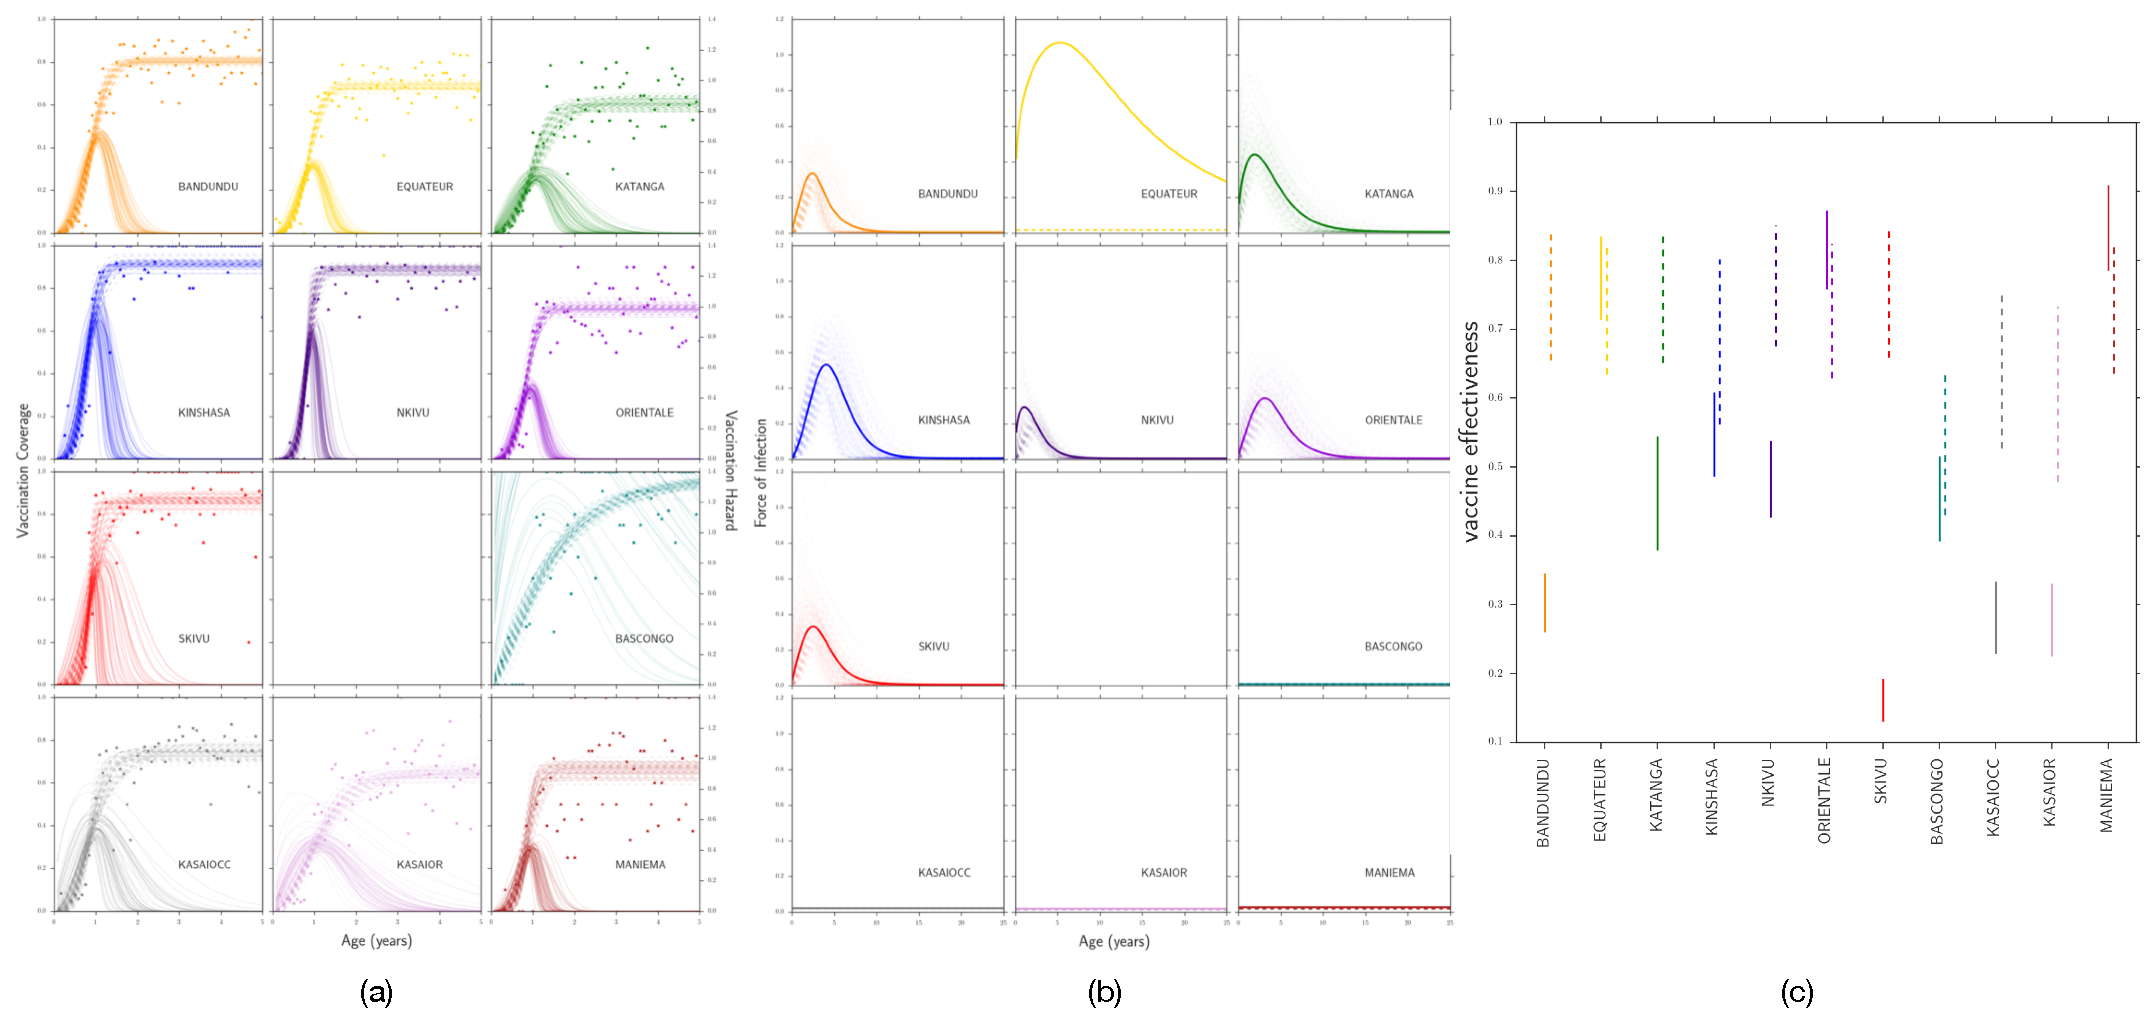
\includegraphics[width=\textwidth,angle=0]{figures/VacFOIveff-crop.pdf}
\caption{\label{fig:foivaccveff} Panel (a): Vaccination hazard (solid lines, right y-axis) and vaccination coverage (dashed lines, left y-axis) recovered using all three sets of data from all 11 provinces, generated from a set of posterior samples. For most provinces, the vaccination hazard is tightly peaked near one year, as expected. Panel (b): The recovered force of infection using all data (solid curve) and only vaccination and case data (dashed curves). As in Figure~\ref{fig:sero}, the solid curve is the mean of the posterior distribution, and the provinces before the blank space were fit using the Weibull plus constant model while those after were fit using the constant-only model for force of infection. In most cases, the inclusion of the serology data did not make a large difference in the inferred force of infection. Panel (c): recovered value for vaccine efficacy ($\pm 1\sigma$) from analyses using all three data sets for each province (solid), and vaccine and case data only (dashed). Note that the values without serology data are almost all consistent with the prior on $\gamma$. Because of our results from the simulated data, we do not expect that these values to reflect the true vaccine efficacy (in general, they are probably biased low), but we \emph{do} expect that the ranking of provinces by vaccine efficacy is correct.}
\end{figure*}

The resulting age-specific hazards for vaccination and FOI illustrate significant province-level variation.  Vaccination at the province-level exhibits strong differences in both the maximum coverage achieved and the timeliness (e.g. the variance of the vaccine hazard - is it tightly peaked or very broad?).  The hazard of vaccination falls to near 0 by approximately 24 months of age in all provinces except for Bas-Congo, where the proportion of children vaccinated continues to increase over the full age range (6-59 months) included in the DHS survey (see Fig.~\ref{fig:foivaccveff}(a)). In the 7 provinces for which the Weibull plus constant FOI hazard was selected, the mode of the fitted FOI was at or below 5 years of age - see Fig.~\ref{fig:foivaccveff}(b).  In 6 of 7 of these provinces, the FOI hazard rate dropped to near 0 by 10 years of age, suggesting little additional infection risk beyond 10 years of age.  In all 7 of these provinces, the fitted hazard rate for the model with and without serology data included were similar.  Equateur province stands out as an exception, here the FOI was highest of all provinces and remained high through adolescence. Notably, the mean age of infection among reported cases was highest in Equateur province. In the 4 provinces for which the constant hazard rate model was preferred, the rates were similar for models analyzed with and without the inclusion of serology data (Fig.~\ref{fig:foivaccveff}(b)).

There was high variability in the estimated vaccine effectiveness in the 11 provinces.  In 8 of 11 provinces, the fitted values are considerably lower than the conventionally assumed vaccine efficacy of ~85\% for measles vaccine~\cite{Uzicanin2011}. Based on the results from the simulation study, above, the absolute value of these estimates should be taken with caution; however, they may reflect a qualitative ranking of effectiveness, or the reliability of vaccination survey responses in these provinces.  The 4 provinces with the lowest values, Bandundu, Sud Kivu, Kasai Occidental, and Kasai Orientale, all reported relatively high vaccination coverage in the 2014 DHS relative to the seroprevalence.  Thus, low effectiveness is consistent with this observation.  Notably, this is corroborated by low estimated effectiveness when the model is analyzed in the absence of serological data  (Fig.~\ref{fig:foivaccveff}(c)).

%In the next figure, Fig.~\ref{fig:foivaccveff}, we examine the vaccination hazard and probability, the force of infection, and the vaccine efficacy for each of the eleven provinces, inferred using all three datasets. The left panel shows the vaccination data as points, the vaccination hazard as solid lines, and the vaccination probability as dashed lines. All curves are generated from samples drawn from the posterior distributions of the model parameters. For almost all of the provinces, the vaccination hazard is peaked tightly around approximately one year in age, as expected. The height of the vacc. hazard corresponds closely to the final level of vaccination probability - higher vaccination hazard means a higher probability of getting vaccinated. The only province that does not follow this pattern is Bas Congo, for which there is evidence for a vaccination hazard with non-negligible weight at higher ages. That is, the probability of being vaccinated is still increasing at the right edge of this graph, which corresponds to five years old.

%The next (middle) panel in Fig.~\ref{fig:foivaccveff} shows the force of infection recovered for each province using all data (solid) and vaccionation/case data (dashed). For all provinces except Equateur, the force of infection is either Weibull plus constant (first seven cells), or constant-only (final four cells) for both datasets. In Equateur, the simpler model is used when vaccination/case data only are used. We see here that all provinces have a non-zero force of infection at higher ages.

%The final (right) panel in Fig.~\ref{fig:foivaccveff} shows the mean value and uncertainty for vaccine efficacy ($\bar{\gamma} \pm \sigma$) for all eleven provinces, with the same color-coding as has been used throughout this section. As expected from the serology results, Sud Kivu has the lowest vaccine efficacy. Because of our results using the simulated data, we believe that the ordering of provinces by $\gamma$ is correct - but we do not believe that the actual values should be taken seriously. From that analysis, we suspect that the recovered values are likely lower than the true values.

\begin{figure}
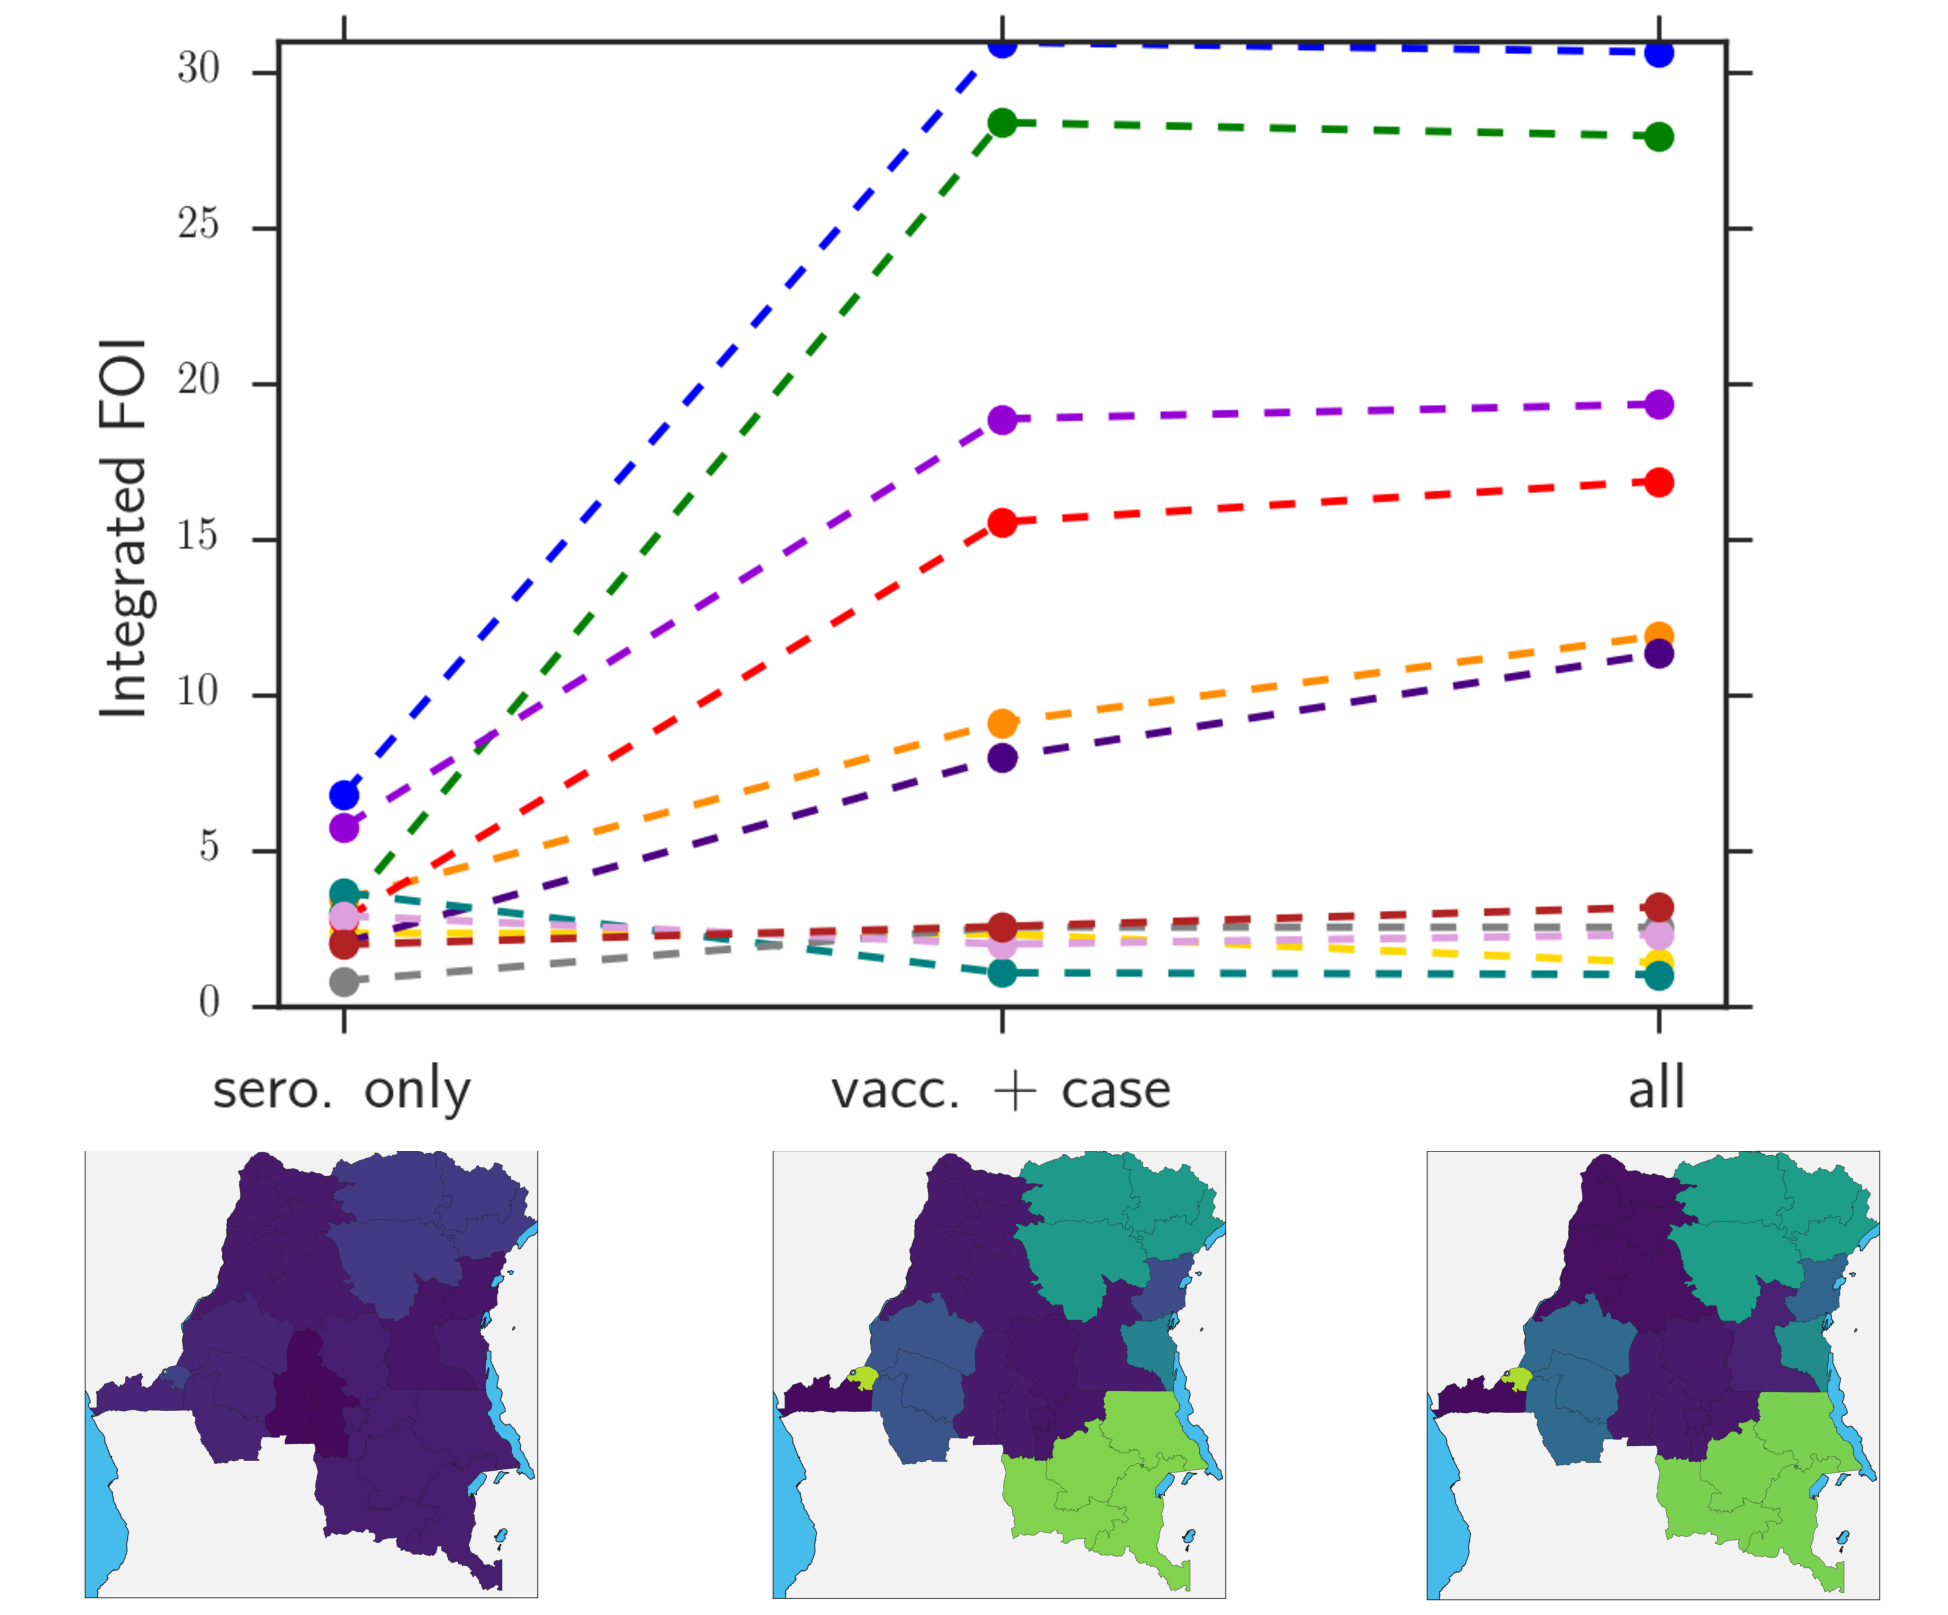
\includegraphics[width=\columnwidth,angle=0]{figures/RiskRank-crop.pdf}
\caption{\label{fig:riskrank} Force of infection integrated to age ten (`risk' )for all eleven provinces, color coded as indicated in Figure~\ref{fig:sero}, calculated using the inferred foi from only serology data (left-most point), case and vaccination data (middle point), and all three datasets. Both the ranking of provinces by risk and the overall values change dramatically between the serology-only and the other two points, but the difference between vaccination plus case and all three data sets is minimal. The maps show the risk in all provinces, with yellow being high risk and dark blue being low risk. }
\end{figure}

%Finally, in Fig.~\ref{fig:riskrank}, we assess what we call the `risk' inferred for with each province, which we define as
%\begin{equation}
%r = \int_0^{10} \mathrm{foi}(a) da,
%\end{equation}
% or the force of infection integrated from 0 to $10$ years. We calculate the foi using serology data only (left-most point), case and vaccination data only (middle point), and all three datasets (right-most point), and show the integrated values in Fig.~\ref{fig:riskrank}. The provinces are color-coded as throughout this section, and a dashed line is drawn to guide the eye between the results for different datasets. Below the points, we show maps of the DRC with each province colored according to the risk level, with dark blue being lowest risk and yellow highest. The most obvious conclusion from this plot is that the inclusion of case and vaccination data leads us to drastically increase our assessment of risk in many provinces. Interestingly, the inclusion of serology data does not make a significant difference in the calculated risk. The information from serology data seems to be most useful for inferring vaccine efficacy, rather than force of infection.

To give a simple summary of the marginal benefit of serology data, we compare estimates of the integrated FOI below 10 years of age from the model fit to age-specific case incidence and vaccination coverage data, to the model including these data plus serological data.  For comparison, we also present the integrated FOI below 10 yars of age when fitting the model to the serological data from the DHS alone.  Using the serology data alone, the estimated integrated FOI is relatively low for all provinces; this result is not surprising as the DHS survey only included data below 59m of age and thus does not provide information for estimating the additional FOI above 59 months of age.  The inclusion of the case data results in higher estimates of the integrated FOI in 7 of 11 provinces.  Notably, while the absolute value of the integrated FOI changes for the full model, including age-specific case, vaccination coverage, and serological data, the rank order does not change relative to the model based on only case and vaccination coverage data. 

\section{Discussion \label{sec:Discussion}}

The age-specific profile of immunity to measles infection can be a powerful tool for the assessment of vaccination programs and the planning for vaccine-based interventions~\cite{CuttsHanson, Winter2018Sero}. Comprehensive serological surveys can be prohibitively expensive and are thus only conducted infrequently.  Age-specific measles case incidence, by contrast, is routinely collected in most national health systems and has been previously used to infer age-specific infection risk via the catalytic model~\cite{griffiths_catalytic_1974, Grenfell1985, farrington_correlated_2013, Ferrari2010FOI}. Here we present a novel extension of the catalytic model that uses age-specific vaccination coverage surveys to account for the competing age-specific rates of immunization via vaccination and natural infection.  We show, using a simulation experiment, that this model can be used to estimate age-specific seroprevalence using age-specific case incidence and vaccination coverage data. A necessary component of this model is the vaccination effectiveness, which gives the proportion of individuals who report vaccination on a survey that are effectively immunized by vaccination.  We show that, while this vaccination effectiveness is difficult to estimate in absolute value, our model-based estimator is positively correlated with the true value used in simulation; thus this estimate may be useful as a relative measure of vaccination effectiveness.  We further show that the inclusion of limited serological survey data, here a survey of children between 6-59 months of age, results in improvements of all model parameters, including vaccination effectiveness. 

We applied our novel catalytic model to age-specific measles case, vaccination survey, and serological survey data from the DRC. The coincidence of a vaccination and serological survey in DRC during the 2014 DHS presents an opportunity to test the model analyzed using only case incidence and vaccination survey data to the directly measured measles seroprevalence. We show that, for most provinces, the age-specific seroprevalence estimated using only age-specific measles case and vaccination survey data is a reasonable approximation of the observed seroprevalence (Fig.~\ref{fig:sero}). We note, however, that the estimated seroprevalence was occasionally biased in a direction that would over-estimate population immunity and under-estimate measles outbreak risk.

The 2014 DHS in DRC included a sero-survey that was limited to children between the ages of 6-59 months. While this survey, by itself, can provide only a limited view of the total population immunity (including individuals older than 59 months) we have shown that combining these data with age-specific case incidence, over all ages, and vaccination coverage data can yield unbiased estimates of the age-specific seroprevalence across all ages, and thus, of the total susceptible population. In most provinces in DRC, these estimates did not differ greatly from those made without the inclusion of the sero-survey; however, in provinces where the estimates based on case incidence and vaccination coverage data only were biased, they tended to over-estimate population immunity.  Thus, even a relatively small investment in serological surveys may have benefits for population-level estimates.  Further, as illustrated in the simulation study, the inclusion of the serological data yields estimates of the vaccination effectiveness that are negatively biased, but preserve the rank order of estimates and thus may provide a useful relative measure of either vaccine program performance or confidence in vaccination coverage surveys.  While it is impossible to definitively identify whether the disparity between coverage and immunity is due to field effectiveness of the vaccine or weak recall in vaccination surveys, the resulting estimate could provide a measure of confidence in vaccine coverage values that may be of use in vaccine planning. The estimates of vaccination effectiveness for the provinces of DRC exhibit wide variation. Bandundu, Sud Kivu, Kasai Occidental, and Kasai Orientale rank as the 4 lowest estimates of vaccination effectiveness.  Again, it is impossible to determine whether this low estimate is due to low performance of the vaccination program or over-estimation of vaccination by mothers during the survey, these results suggest the value of further evaluation in these regions to evaluate vaccination levels. 

This study has several limitations that should be considered when interpreting these results.  The first set of limitations pertain to the assumptions of the catalytic model. An implicit assumption of the catalytic model (and previous incarnations of the catalytic model~\cite{griffiths_catalytic_1974, Grenfell1985, whitaker_estimation_2004} is that both the vaccination and FOI hazards have been fixed and constant in the past.  This assumption is almost certainly violated in practice as coverage with measles containing vaccine has been increasing in most countries in the world~\cite{perry_global_2014}; thus, while the shape of the vaccine hazard may remain constant, the magnitude is likely to be increasing.  This implies that the fitted hazard is a reflection of the vaccination hazard over recent time, rather than current vaccination.  Similarly, we would expect the magnitude of FOI would be negatively correlated with vaccination coverage, and thus would be declining over time, rather than constant.  We note that in our simulations, vaccination coverage increased linearly over time from the time of introduction to the time of sampling and the fits to the simulated data still gave reasonable estimates of the age-specific seroprevalence at the time of sampling. In addition, the model, as we have stated it here does not formally account for the additional immunity in specific age cohorts that would result from pulsed, age-targeted vaccination campaigns (SIAs). We note that it is possible to include such pulsed campaigns in such an analysis per methods described in [Li et al PLoS Med].

A second set of assumptions arise from the inherent limitations of surveillance and survey data. As highlighted in the definition of the vaccination effectiveness parameter, $\gamma$, vaccination surveys often rely on maternal recall, which is frequently non-specific and may suffer from recall bias.  This results in the indeterminacy of the vaccination effectiveness parameter as a measure of field effectiveness of the vaccine or the reliability of vaccine survey responses. In the specific case of measles, there are multiple potential sources of vaccination -- routine immunizations and multiple types of supplemental activities that range from child-maternal health days to SIAs to outbreak response vaccination campaigns. The vaccination hazard estimated here is not specific to any of these because the vaccination question in the DHS survey is not specific to any one source of vaccination~\cite{takahashi_geography_2017, metcalf_transport_2015}.  Thus, the vaccination hazard reflects the sum of all sources of vaccination. The age-specific case surveillance reflects only those cases that were recorded in the health system and may contain biases if, for example, younger children are more likely to be taken to clinics or hospitals because of more severe disease. 

Though comprehensive serological surveys remain the gold-standard for estimating the age-distribution of immunity, our analysis suggests that reasonable estimates of seroprevalence may be possible by combining vaccination coverage surveys and routinely collected age-specific case reports.  In particular, this may allow initial estimates of seroprevalence that could be used to support the design of serological surveys.  Further, these methods would permit evaluation of population immunity in years when sero-surveys are not available.  As illustrated in the simulation experiment, the combination of limited serological surveys, here only 6-59 months of age, with routine surveillance data may allow robust estimates of population immunity and evaluation of vaccination program performance, through the vaccination effectiveness parameter.  Thus, by combining serological surveys with existing surveillance data, it may be possible to obtain operationally useful estimates using smaller and less expensive survey designs.  The development of optimal survey designs (age ranges and sample sizes) to estimate population immunity by combining sero-surveys with surveillance is a useful avenue for future research.


%Discussion:

%Application for estimating seroprevalence in settings where a sero-survey is not possible 
%	? serosurvey may not be feasible to do frequently, but this allows us to use passively collected age-specific case incidence 
%	? doing a very wide serosurvey may not be feasible, or practical, but case surveillance lets you see signal across a wide age range

%What is the use of this?
%	? estimating seroprevalence in the absence of surveys
%	? effect size estimate for designing sero-surveys

%Discuss the interpretation of the patterns seen in the DRC data 
%	? which places have good vaccination, which have high transmission
%	? As I recall, some provinces have very wide FOI hazards, indicating that some people are getting infected relatively late in life.  There are lots of possible reasons for this, so should give it some thought.  Could relatively low exposure, so some people are just not exposed until late in life.  Could also reflect inflow of internally displaced people (IDPs).  Speculation depends on the pattern. 

%Several things that we haven?t dealt with here, that we?ll need to at least acknowledge:
%	- we haven?t dealt with the fact that incidence and vaccination are not stationary
%	- we haven?t dealt with supplemental campaigns
%	- these are all things that can be dealt with at least theoretically

%Take-home message about merging serosurveillance and case-based surveillance

\appendix*
    \section{Full Results from MCMC Runs}
Here, in Figure~\ref{fig:cornerplot}, we show the two-dimensional posterior distributions for all pairs of parameters from the MCMC runs on the DRC data. The correlation patterns between the different parameters are typically quite simple, except for that between $v_\alpha$ and $v_\beta$ and that between $f_\eta$ and $\omega$, both of which exhibit curvature. There is no indication that the sampler was unable to explore the full parameter space.

It is also worth noting in this Figure that Equateur (in yellow) in general has parameter values that are outliers from the other provinces. This is possibly an indicator of why Equateur was the only province that was best described by the more complicated model when fitting all three datasets, but by the simpler model when using only case and vaccination data.

\begin{figure*}
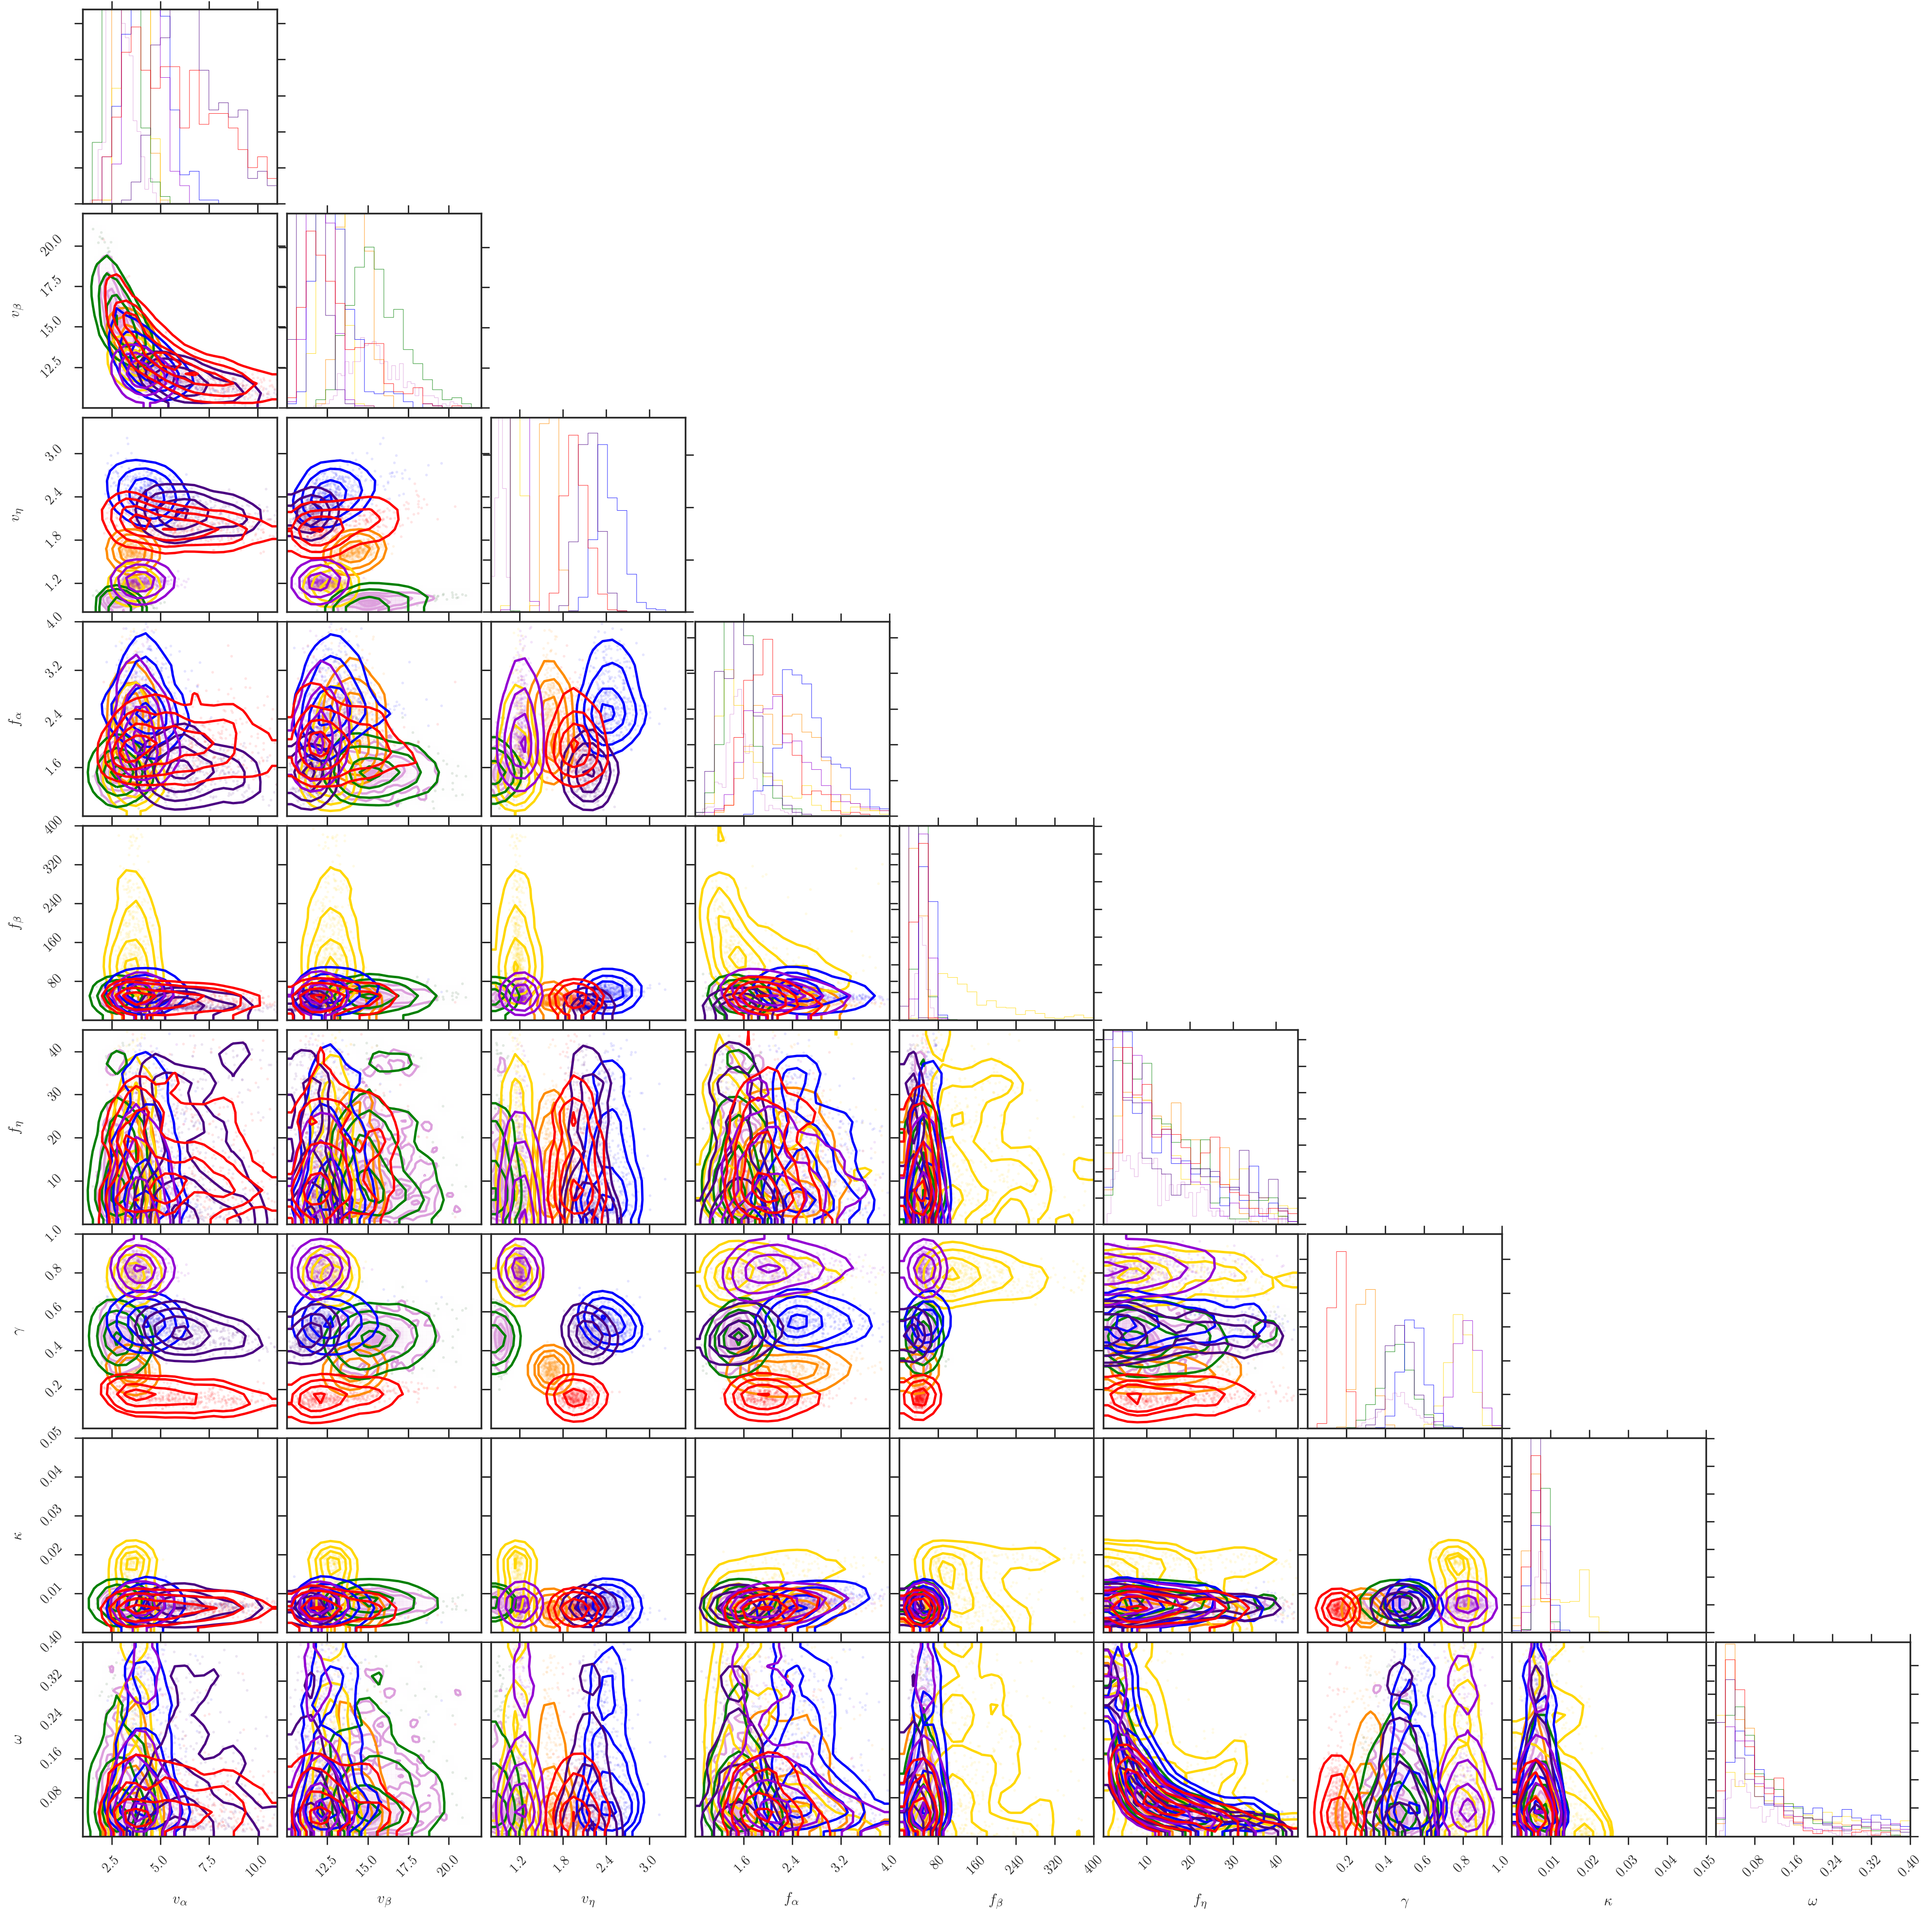
\includegraphics[width=\textwidth,angle=0]{figures/cornerplot.png}
\caption{\label{fig:cornerplot}  Two-dimensional posterior distributions for all pairs of parameters for the seven provinces that were best described by the more complicated force of infection model. The correlation structure between the different parameters is simple with a few exceptions.}
\end{figure*}


\bibliographystyle{unsrt}
\bibliography{master}

\end{document}







